\section{Préparation du projet}

\begin{frame}{Préparation du projet}
  % TODO: Objectif: -> mettre en place le maximum de bonnes pratiques
  \begin{block}{Étapes}
    \begin{itemize}
    \item Collecte des exigences du client.
    \item Tests et documentation.
    \item Normes et qualité.
    \end{itemize}
  \end{block}
\end{frame}

\begin{frame}{Exigences fonctionnelles}

  \begin{block}{Une liste des exigences fonctionnelles}
    \begin{itemize}
    \item Conception \textbf{conforme à la maquette} comprenant:
      \begin{itemize}
      \item une barre de navigation,
      \item une vignette présentant le meilleur film,
      \item une catégorie des films les mieux notés,
      \item trois catégories aux choix comprenant sept films.        
      \end{itemize}
    \item \textbf{Informations d'un film} \textit{via} une fenêtre
      modale contenant:
      \begin{itemize}
      \item l'image, le titre, le genre, la date de sortie,
      \item le classement, le score IMDB,
      \item le réalisateur, les acteurs,
      \item la durée, la pays d'origine, le résultat au \textit{box
        office} et
      \item le résumé du film.
      \end{itemize}
    \end{itemize}
  \end{block}
\end{frame}

\begin{frame}{Exigences non-fonctionnelles}
  \begin{block}{Une liste des exigences non-fonctionnelles}
    \begin{itemize}
    \item \textbf{Portabilité} vers les navigateurs Chrome, Safari et Firefox.
    \item Utilisation de l'API \textbf{OCMovies-API} et accès \textit{via} des requêtes AJAX.
    \item \textbf{Mise-à-jour automatique} des données.
    \item Utilisation de Javascript et de CSS \textbf{sans \textit{framework} ni bibliothèque}.
    \end{itemize}
  \end{block}
\end{frame}

\begin{frame}{Tester le \textit{front-end}}

  % SRC: https://npmcompare.com/compare/chai,jasmine,jest,karma,mocha
  % - jasmine has fewer dependencies, fewer open issues and fewer open
  % pull requests.
  % - jest has more versions, more frequent updates, a
  % bigger community of maintainers, more daily downloads, more weekly
  % downloads, more monthly downloads, more stars on Github, more
  % followers on Github and more forks
  % - mocha has been out there for longer
  % -> Choix de jasmine

  \only<1> {
    \begin{block}{Pourquoi tester le \textit{front-end} ?}
      \begin{itemize}
      \item Vérifier que le produit est conforme aux exigences.
      \item Mettre en place des vérifications pour accompagner une
        potentielle future mise à l'échelle.
      \item Documenter les bugs et éviter autant que possible les
        régressions.
      \end{itemize}
    \end{block}
  }
  
  \only<2>{
    \begin{block}{Utilisation de Mocha}
      Choix d'utiliser Mocha car\footnote{Voir \url{https://npmcompare.com/compare/chai,jasmine,jest,karma,mocha}}:
      \begin{itemize}
      \item Est simple d'utilisation.
      \item Est flexible.
      \item $\rightarrow$ Prend peu de place au sein du projet.
      \end{itemize}
    \end{block}
  }
  
\end{frame}

\begin{frame}{Documenter le \textit{front-end}}
  \begin{block}{Pourquoi documenter le \textit{front-end} ?}
    \begin{itemize}
    \item Le projet peut être repris à l'avenir par quelqu'un d'autre.
    \item Le projet peut grossir et se complexifier.
    \end{itemize}
  \end{block}

  \begin{block}{Utilisation de JSDoc}
    Choix d'utiliser JSDoc car:
    \begin{itemize}
    \item facile et rapide à installer,
    \item facile à utiliser,
    \item génère une documentation claire et concise.
    \end{itemize}
  \end{block}

\end{frame}

\begin{frame}{Normes et qualité}
  \only<1>{
    \begin{block}{Vérifier le code HTML}
      \begin{itemize}
      \item Permet de détecter les erreurs dans le code HTML.
      \item Permet de garantir la conformité du code avec les recommandations de la W3C\footnote{World Wide Web Consortium}.
      \item Disponible sous forme d'extension pour navigateurs\footnote{Disponible au moins pour Chrome et Firefox.}.
      \end{itemize}
    \end{block}
  }

  \only<2> {
    \begin{figure}
      \begin{center}
        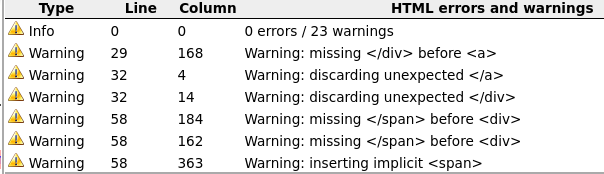
\includegraphics[scale=0.45]{../../res/html_validator.png}
      \end{center}
      \caption{HTML Validator: une extension firefox pour vérifier le code HTML}    
    \end{figure}
  }

  \only<3> {
    \begin{block}{Vérifier le code Javascript}
      Utilisation de ESLint\footnote{\url{https://eslint.org/}}, un \textit{linter} pour Javascript.
      \begin{itemize}
      \item Permet de localiser les erreurs javascript.
      \item Permet également de localiser les erreurs de style.
      \item Permet de générer un rapport.
      \end{itemize}
    \end{block}
  }

  \only<4> {
    \begin{figure}
      \begin{center}
        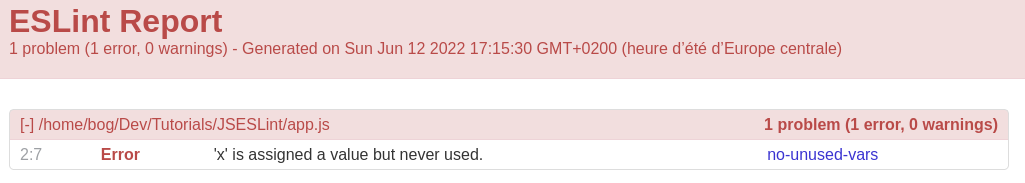
\includegraphics[scale=0.3]{../../res/eslint.png}
      \end{center}
      \caption{Exemple de rapport généré par ESLint.}      
    \end{figure}
  }
\end{frame}
